\section{Lab: Locks}

\subsection{实验目的}
本实验将重新设计代码以提高并行性。多核机器上并行性差的一个常见症状是高锁争用。提高并行性通常涉及更改数据结构和锁定策略以减少争用。实验将为 xv6 内存分配器和块缓存执行此操作。

\subsection{实验步骤}

\subsubsection{优化Memory allocator}

修改系统对内存的管理方式。修改后,物理内存的分配和释放通过一系列链表进行管理,这些链表称为空闲链表(freelist),每个链表节点代表一块空闲的物理内存。

系统为每个 CPU 分配了一个单独的空闲链表,并为每个链表分配了一个自旋锁,以确保在多核环境下的同步操作。每当内存需要释放时,内存管理器会将内存块插入到相应 CPU 的空闲链表的头部。这个操作受 CPU 的自旋锁保护,以避免在并发情况下的数据竞争。内存分配时,首先会尝试从当前 CPU 的空闲链表中获取空闲页面,如果当前 CPU 的链表为空,则尝试从其他 CPU 的链表中窃取一个页面。

具体来说,就是对kalloc.c文件进行修改,以应用这种内存管理的方式。修改如下:
\begin{enumerate}
    \item 修改kmem结构体,把它改为数组的形式,以便将其拆分到每个CPU中。
          \begin{lstlisting}[language=c,title=对kmem结构体的修改]
    // kmem 是一个包含 NCPU 个元素的数组,每个元素对应一个 CPU 的物理内存管理结构。
    // 其中 lock 是自旋锁,用于保护空闲链表 freelist。
    struct
    {
        struct spinlock lock; // 自旋锁,用于多核环境下的同步。
        struct run *freelist; // 空闲链表,指向空闲内存块。
    } kmem[NCPU];           // 定义 NCPU 个这样的结构体数组。
    \end{lstlisting}
    \item 修改kinit函数,初始化空闲链表。
          \begin{lstlisting}[language=c,title=对kinit函数的修改]
    // 初始化内存分配器
    void kinit()
    {
        char lockname[16]; // 用于存储锁的名字。
        for (int i = 0; i < NCPU; i++)
        {
        // 为每个 CPU 初始化一个自旋锁,并给它们命名。
        snprintf(lockname, sizeof(lockname), "kmem_CPU%d", i);
        initlock(&kmem[i].lock, lockname);
        }
        // 将从内核结束位置(end)到物理内存顶(PHYSTOP)之间的内存标记为空闲。
        freerange(end, (void *)PHYSTOP);
    }    
    \end{lstlisting}
    \item 修改kfree,把释放后的内存加入空闲链表。
          \begin{lstlisting}[language=c,title=对kfree函数的修改]
    void kfree(void *pa)
    {
        struct run *r; // 临时指针,用于指向将要释放的内存块。
        int cpu_id;    // 存储当前 CPU 的 ID。
    
        // 如果 pa 不是页面对齐的,或地址超出合法范围,则触发 panic。
        if (((uint64)pa % PGSIZE) != 0 || (char *)pa < end || (uint64)pa >= PHYSTOP)
        panic("kfree");
    
        // 将内存填充为 1,以捕捉潜在的悬空引用(dangling references)。
        memset(pa, 1, PGSIZE);
    
        r = (struct run *)pa; // 将 pa 转换为 run 结构体类型。
    
        push_off();       // 关闭中断,防止在获取 CPU ID 时发生上下文切换。
        cpu_id = cpuid(); // 获取当前 CPU 的 ID。
        pop_off();        // 恢复中断。
    
        acquire(&kmem[cpu_id].lock);     // 获取当前 CPU 对应的自旋锁。
        r->next = kmem[cpu_id].freelist; // 将释放的内存块插入空闲链表的头部。
        kmem[cpu_id].freelist = r;       // 更新空闲链表的头指针。
        release(&kmem[cpu_id].lock);     // 释放自旋锁。
    }    
    \end{lstlisting}
    \item 修改kalloc,完善从其他CPU窃取空闲空间的机制。
          \begin{lstlisting}[language=c,title=对kalloc函数的修改]
    // 分配一个 4096 字节的物理内存页面。
    // 返回一个内核可以使用的指针。如果无法分配内存,则返回 0。
    void *kalloc(void)
    {
        struct run *r; // 临时指针,用于指向将要分配的内存块。
        int cpu_id;    // 存储当前 CPU 的 ID。
    
        push_off();       // 关闭中断,防止在获取 CPU ID 时发生上下文切换。
        cpu_id = cpuid(); // 获取当前 CPU 的 ID。
        pop_off();        // 恢复中断。
    
        acquire(&kmem[cpu_id].lock); // 获取当前 CPU 对应的自旋锁。
        r = kmem[cpu_id].freelist;   // 从空闲链表中取出第一个空闲块。
        if (r)
        {
        kmem[cpu_id].freelist = r->next; // 更新空闲链表的头指针。
        }
        else
        {
        // 如果当前 CPU 的空闲链表为空,则尝试从其他 CPU 的空闲链表中窃取空闲块。
        for (int i = 0; i < NCPU; i++)
        {
            if (i == cpu_id)
            continue;             // 跳过当前 CPU 自己。
            acquire(&kmem[i].lock); // 获取其他 CPU 对应的自旋锁。
            r = kmem[i].freelist;   // 尝试从其他 CPU 的空闲链表中获取空闲块。
            if (r)
            kmem[i].freelist = r->next; // 更新空闲链表的头指针。
            release(&kmem[i].lock);       // 释放自旋锁。
            if (r)
            break; // 如果成功获取到空闲块,则跳出循环。
        }
        }
        release(&kmem[cpu_id].lock); // 释放当前 CPU 的自旋锁。
    
        if (r)
        memset((char *)r, 5, PGSIZE); // 捕捉潜在的错误。
        return (void *)r;               // 返回分配的内存块指针。如果分配失败,则返回 0。
    }            
    \end{lstlisting}
\end{enumerate}

\subsubsection{优化Buffer cache}

修改bio.c文件,将缓冲区缓存划分为多个桶,并为每个桶分别设置独立的锁,使得不同线程可以并发地访问不同桶内的缓冲区,减少了锁的竞争。此外,全局锁只在需要确保缓存整体一致性时才短暂持有,大部分操作仅需获取局部的桶锁,进一步降低了锁竞争的发生频率。

\begin{enumerate}
    \item 在buf.h文件中修改缓冲区结构体,添加一个记录缓冲区最后使用时间的成员。
          \begin{lstlisting}[language=c,title=buf.h的修改]
    struct buf
    {
        int valid; // has data been read from disk?
        int disk;  // does disk "own" buf?
        uint dev;
        uint blockno;
        struct sleeplock lock;
        uint refcnt;
        struct buf *prev; // LRU cache list
        struct buf *next;
        uchar data[BSIZE];
        uint last_used_tick;
    };
    \end{lstlisting}
    \item 在param.h文件中添加一个NBUCKET常量,按照提示设为质数13,作为哈希表的桶的数量。
          \begin{lstlisting}[language=c,title=添加常量]
    #define NBUCKET 13
        \end{lstlisting}
    \item 修改bio.c文件,优化缓冲区的操作方式:
          \begin{itemize}
              \item 修改缓冲区缓存结构体,将其改为哈希表形式,并为每一个桶设置一个锁。
                    \begin{lstlisting}[language=c,title=对缓冲区缓存结构体的修改]
    // 缓冲区缓存结构体
    struct
    {
        struct spinlock lock[NBUCKET]; // 每个桶(bucket)一个锁,用于保护桶中的缓冲区链表。
        struct buf buf[NBUF];          // 缓冲区数组,存放 NBUF 个 buf 结构体。
        struct spinlock bcache_lock;   // 用于保护整个缓存的锁。
    
        // 所有缓冲区的链表,通过 prev/next 连接。
        // 链表按照缓冲区最近使用的时间排序。
        // head.next 是最近使用的缓冲区,head.prev 是最久未使用的缓冲区。
    
        struct buf head[NBUCKET]; // 每个桶都有一个链表头节点。
    } bcache;
              \end{lstlisting}
              \item 修改binit函数,增加哈希表的初始化操作。
                    \newpage
                    \begin{lstlisting}[language=c,title=对binit函数的修改]
    void binit(void)
    {
        struct buf *b;

        // 初始化全局缓存锁
        initlock(&bcache.bcache_lock, "bcache_lock");

        // 初始化每个桶的锁
        for (int i = 0; i < NBUCKET; ++i)
        {
            initlock(&bcache.lock[i], "bcache_bucket");
        }

        // 初始化每个桶的链表头节点,指向自己,表示链表为空
        for (int i = 0; i < NBUCKET; ++i)
        {
            bcache.head[i].prev = &bcache.head[i];
            bcache.head[i].next = &bcache.head[i];
        }

        // 初始化每个缓冲区并将其插入到第一个桶的链表中
        for (b = bcache.buf; b < bcache.buf + NBUF; b++)
        {
            b->next = bcache.head[0].next;
            b->prev = &bcache.head[0];
            initsleeplock(&b->lock, "buffer"); // 初始化缓冲区的睡眠锁
            bcache.head[0].next->prev = b;
            bcache.head[0].next = b;
        }
    }
              \end{lstlisting}
              \item 修改bget函数,修改缓冲区的查找和分配方式。
                    \begin{lstlisting}[language=c,title=对bget函数的修改]
    static struct buf * bget(uint dev, uint blockno)
    {
        struct buf *b;
        int index = blockno % NBUCKET; // 根据块号计算桶的索引

        // 加锁,遍历当前桶的链表,查找指定的缓冲区
        acquire(&bcache.lock[index]);

        for (b = bcache.head[index].next; 
        b != &bcache.head[index]; 
        b = b->next)
        {
            if (b->dev == dev && b->blockno == blockno)
            {
                // 找到目标缓冲区,增加引用计数并释放桶的锁
                b->refcnt++;
                release(&bcache.lock[index]);
                acquiresleep(&b->lock); // 获取缓冲区的睡眠锁
                return b;
            }
        }
        release(&bcache.lock[index]); // 未找到,释放桶的锁

        // 全局加锁,防止其他进程同时修改缓冲区缓存
        acquire(&bcache.bcache_lock);
        acquire(&bcache.lock[index]); // 重新获取桶的锁

        // 再次查找缓冲区,防止在加锁前其他进程已分配该缓冲区
        for (b = bcache.head[index].next; 
        b != &bcache.head[index]; 
        b = b->next)
        {
            if (b->dev == dev && b->blockno == blockno)
            {
                b->refcnt++;
                release(&bcache.lock[index]);
                release(&bcache.bcache_lock);
                acquiresleep(&b->lock);
                return b;
            }
        }

        // 查找最近最少使用的(LRU)缓冲区块
        struct buf *lru_block = 0;
        int min_tick = 0;
        for (b = bcache.head[index].next; 
        b != &bcache.head[index]; 
        b = b->next)
        {
            if (b->refcnt == 0 && 
            (lru_block == 0 || b->last_used_tick < min_tick))
            {
                min_tick = b->last_used_tick;
                lru_block = b;
            }
        }

        // 如果找到LRU块,则将其初始化并返回
        if (lru_block != 0)
        {
            lru_block->dev = dev;
            lru_block->blockno = blockno;
            lru_block->refcnt++;
            lru_block->valid = 0;

            release(&bcache.lock[index]);
            release(&bcache.bcache_lock);

            acquiresleep(&lru_block->lock);
            return lru_block;
        }

        // 如果当前桶没有可用的缓冲区,则尝试从其他桶中窃取缓冲区
        for (int other_index = (index + 1) % NBUCKET; 
        other_index != index; 
        other_index = (other_index + 1) % NBUCKET)
        {
            acquire(&bcache.lock[other_index]);
            for (b = bcache.head[other_index].next; 
            b != &bcache.head[other_index]; 
            b = b->next)
            {
                if (b->refcnt == 0 && 
                (lru_block == 0 || b->last_used_tick < min_tick))
                {
                    min_tick = b->last_used_tick;
                    lru_block = b;
                }
            }

            // 如果找到LRU块,则将其重新插入到当前桶中并返回
            if (lru_block)
            {
                lru_block->dev = dev;
                lru_block->refcnt++;
                lru_block->valid = 0;
                lru_block->blockno = blockno;

                lru_block->next->prev = lru_block->prev;
                lru_block->prev->next = lru_block->next;
                release(&bcache.lock[other_index]);

                lru_block->next = bcache.head[index].next;
                lru_block->prev = &bcache.head[index];
                bcache.head[index].next->prev = lru_block;
                bcache.head[index].next = lru_block;
                release(&bcache.lock[index]);
                release(&bcache.bcache_lock);

                acquiresleep(&lru_block->lock);
                return lru_block;
            }
            release(&bcache.lock[other_index]);
        }

        // 如果所有桶都没有可用缓冲区,则触发 panic
        release(&bcache.lock[index]);
        release(&bcache.bcache_lock);
        panic("bget: no buffers");
    }
              \end{lstlisting}
              \item 修改brelse函数,修改缓冲区的释放方式。
                    \begin{lstlisting}[language=c,title=对brelse函数的修改]
    // 释放已锁定的缓冲区。
    // 将其移动到最近使用的链表头。
    void brelse(struct buf *b)
    {
        if (!holdingsleep(&b->lock)) // 检查是否持有缓冲区的睡眠锁
            panic("brelse");

        releasesleep(&b->lock); // 释放睡眠锁

        acquire(&bcache.lock[b->blockno % NBUCKET]);
        b->refcnt--; // 减少引用计数
        if (b->refcnt == 0)
        {
            b->last_used_tick = ticks; // 更新缓冲区最后使用的时间
        }

        release(&bcache.lock[b->blockno % NBUCKET]);
    }
              \end{lstlisting}
          \end{itemize}
\end{enumerate}

\subsection{评测结果}

利用grade-lab-lock脚本评测,得到结果如图\ref{fig:lock}。
\begin{figure}[ht]
    \centering
    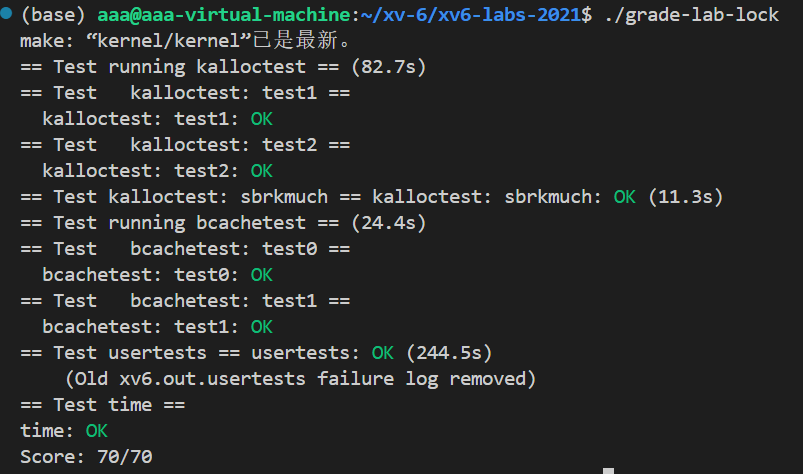
\includegraphics[width=\linewidth]{pics/lock评测结果.png}
    \caption{评测结果}
    \label{fig:lock}
\end{figure}

\subsection{实验小结}

在本次实验中,我通过对xv6系统中的内存分配器和缓冲区缓存机制进行优化,成功地提高了系统的并行性。实验的优化策略主要集中在减少锁的争用,提高系统的并行处理能力。结果表明,通过这些优化措施,系统在多核环境下的性能得到了显著提升,锁的争用情况得到了明显缓解。评测结果也验证了我的优化方案在实践中的有效性。

总的来说,本次实验通过对锁争用问题的深入分析和针对性的优化,展示了提高并行性的重要性和实现方法。未来的工作可以继续探索其他可能的优化点,例如进一步精细化锁的粒度,或是引入更高级的锁机制,以进一步提升系统的并行处理能力。






